% Cita textual seccion Desarrolo:

% Deben explicarse los metodos numericos que utilizaron
% y su aplicacion al problema concreto involucrado en el trabajo practico.
% Se deben mencionar los pasos que siguieron para implementar
% los algoritmos, las dificultades que fueron encontrando y la
% descripcion de como las fueron resolviendo.

% Explicar tambien como fueron planteadas y realizadas las
% mediciones experimentales. Los ensayos fallidos, hipotesis y
% conjeturas equivocadas, experimentos y metodos malogrados deben
% figurar en esta seccion,
% con una breve explicacion de los motivos de estas fallas
% (en caso de ser conocidas).

% Template de matriz
% \[
% \begin{bmatrix} % Matriz con linea rectangular
% \begin{pmatrix} % Matriz con linea redonda
%     x_{11} & x_{12} & x_{13} & \dots  & x_{1n} \\
%     x_{21} & x_{22} & x_{23} & \dots  & x_{2n} \\
%     \vdots & \vdots & \vdots & \ddots & \vdots \\
%     x_{d1} & x_{d2} & x_{d3} & \dots  & x_{dn}
% \end{pmatrix}
% \end{bmatrix}
% \]

\section{Calibración}

\todo[inline] {Mejorar intro}
\todo[inline]{Que es y por que tuvimos que hacerlo. Contar como necesitamos esto para aplicarlo al resto del trabajo practico}
\todo[inline]{Explicar como obtenemos ciertos datos (centro y punto mas iluminado)}
\todo[inline]{Explicar la idea teorica de la calibracion, incluir grafico esfera para ilustrar}
\todo[inline]{Escribir lindas las cuentas de los despejes}
\todo[inline]{En la seccion de experimentacion se vera como diffieren con las dadas por la catedra}

Queremos calcular las normales en cada punto de la superficie.
Tomando 3 imagenes diferentes (por ej 1, 2 y 3), utilizamos las luces $s_{algo}$ y las intensidades registradas $I_{algo}$ para calcular los $m_{algo}$ que son $tal cosa$.
Los $I_{algo}$ podemos obtenerlos $asi y asa$, que es sencillo. No es tan trivial el calculo de los $s_{algo}^{i}$.

Es decir, necesitamos resolver el siguiente sistema: \\

\[
% \begin{bmatrix} % Matriz con linea rectangular
\begin{pmatrix}
    s_{x}^{1} & s_{y}^{1} & s_{z}^{1} \\
    s_{x}^{2} & s_{y}^{2} & s_{z}^{2} \\
    s_{x}^{3} & s_{y}^{3} & s_{z}^{3}
\end{pmatrix}
% \end{bmatrix}
\begin{pmatrix}
    m_{x} \\
    m_{y} \\
    m_{z}
\end{pmatrix}
=
\begin{pmatrix}
    I_{1} \\
    I_{2} \\
    I_{3}
\end{pmatrix}
\]


Tenemos que $S = (s_{x}^{i}, s_{y}^{i}, s_{z}^{i})$ es el vector luz en la imagen $i$. Dado que vamos a explicar el cálculo para una imagen cualquiera, omitiremos el supraíndice $i$ para una notación mas relajada.

Llamemos $c = (c_{x}, c_{y}, c_{z})$ al centro de la esfera. Pensemos la luz como un vector que apunta hacia el centro. El vector $S$ toca la superficie en un cierto punto $p = (p_{x}, p_{y}, p_{z})$, pero $p$ no es un punto al azar, sino que es el punto más iluminado de la esfera. \\

{\centering
    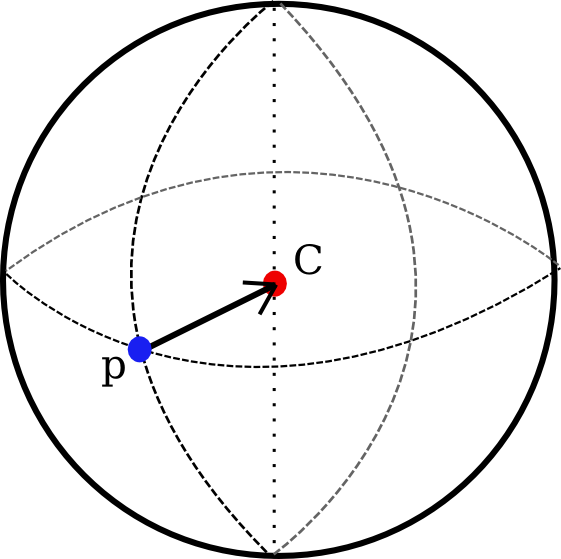
\includegraphics[scale=0.9]{informe/imagenes/esfera/esferaModelo.png} \\
}

El vector $S$ que buscamos es el que va de $p$ a $c$, Por lo tanto

Los vectores que buscamos son de la forma (cx - py, cy - py, cz - pz)

Sabemos el centro y el radio del eje x e y por esto y esto. (Mostrar imagen)
Utilizando la magia de la esfera, veamos como podemos hacerlo
(mostrar cuenterio)



\section{Métodos}

\subsection{Eliminación Gaussiana}

\todo[inline]{Hablar del algoritmo}
\todo[inline]{Explicar por que podemos aplicarlo con las luces, decir que las 3 que tomamos son li entonces no pincha nunca}

\subsection{LU}
\todo[inline]{Que es esto}
\todo[inline]{Por que nos sirve para nuestro problema, hablar de repeticion de calculos}

\subsection{Cholesky}
\todo[inline]{algo}


\section{Cálculo de normales}

\todo[inline]{Explicar que es lo que tenemos que resolver}
\todo[inline]{Explicar como aplicamos los metodos listados arriba para resolver el problema, y por que podemos hacerlo}


\section{Estimacion de profundidades}

\todo[inline]{Hablar del ultimo sistema de ecuaciones de la cual (aun) no tengo idea}


\section{Resultados}
\todo[inline] {Dar imagenes minimo del resultado final}



\section{Experimentación}

\todo[inline]{PENSAR MAS}
\todo[inline]{Mostrar como con diferentes luces obtenemos diferentes normales}
\todo[inline]{Diferencias de tiempos EG vs LU vs mascara y combinaciones}

